Fundamentally, the optical layout in HAM6 must combine the signal beam and the \gls{lo} beam and sense the combined beams to form a \gls{bhd}. The location of HAM6 with respect to the rest of the interferometer is shown in Figure~\ref{fig:ligolayout}. As loss, such as that caused by mode mismatch, in the interferometer's readout will degrade its sensitivity, and as there is uncertainty in the interferometer's beam parameter, it is vital that the \gls{awc} can correct for possible mode mismatches between the interferometer and the \glspl{omc} so that loss due to mode mismatch is minimal.
\par
In this chapter, the effectiveness of the \gls{awc} is analysed. Figure~\ref{fig:bhdforligochapterlayout5fmodessrmomcmode matchingsuccess} shows the range of modes at the \gls{srm} which can be corrected for such that the target for loss due to mode mismatch for A+ can be met. Other aspects of this layout and its requirements outside the scope of this thesis can be found in~\cite{CDR_BHD,BHD_ISC_requirements}.
%\par
%In Section~\ref{sec:bhd_for_ligo_chosen_layout}, the optical properties of the proposed HAM6 layout are examined. Section~\ref{sec:BHD_for_ligo_WS_visulations} is an analysis of how mode mismatches between the interferometer and the OMC can be corrected by the \gls{awc}. Section~\ref{sec:BHD_for_ligo_conclusion} is the conclusion for this chapter.
\section{The Optics for Mode Matching the Interferometer and the Output Mode Cleaners}
\label{sec:bhd_for_ligo_chosen_layout}
The design of the optical layout within HAM6 that is being taken forward\footnote{As of January 2021, millimetre scale changes have been made which do not affect the analysis in this chapter.} is shown in Figure~\ref{fig:bhdforligochapterlayout5f}. The properties of this layout are summarised in Table~\ref{tab:layout_parameters}. The two beam paths after the beam splitter upon which the signal and \gls{lo} beams are combined (BHDBS2) are called A and B. The mirrors OMA1, OMB1, OMA2 and OMB2 will be referred to as OMx1 and OMx2 as it is not important to make a distinction between the A and B paths when considering mode matching. The A/B paths are terminated by OMCA/B.
\begin{figure}
	\centering
	
\includegraphics[width=0.95\linewidth]{BHD_for_ligo_HAM_6_layout.eps}
	\caption[Sketch of the balanced homodyne detection scheme for LIGO A+.]{The \gls{lo} beam enters HAM6 directly above BHDBS2 (north side), and it is highlighted in green. The signal beam enters HAM6 directly above OM0 (north side), and it is highlighted in pink. The signal beam is steered by OM0 onto BHDBS2 where it is combined with the \gls{lo}. The two combined beams are shown in red. These are incident upon a mirror used for steering (OMxS), and then upon two curved mirrors (OMx1 and OMx2). The beams enter the \glspl{omc}, which are seismically isolated by the BHSS (the large triangular component). The spacings for these components are given in Table~\ref{tab:layout_parameters}.}
	\label{fig:bhdforligochapterlayout5f}
\end{figure}
\par
The \gls{awc} in HAM6 has two functions: it will be used to correct for errors in the interferometer's beam parameter at the SRM, e.g.~due to thermal effects or errors in the \gls{roc} of the optics in the \gls{src}, and to correct for geometry errors within HAM6 such that the mode matching between the arm mode and the \gls{omc} is maximised~\cite{BHD_ISC_requirements}. As mentioned in Section~\ref{sec:beam_parameter_chapter_mm_losses}, the loss in sensitivity from mode mismatch can be four times greater than a simpler source of loss (e.g.~photodiode quantum efficiency) due to coherent destructive modal interference~\cite{McCuller2020a}. Active mirrors, called \gls{sams}, will be used to correct for mode mismatch; they will provide a range of at least $\pm50$\,mD of optical power~\cite{SAMS_DesignRequirementsDocument}.
\par
The optical layout in HAM6 must mode match the nominal \gls{srm} and \gls{omc} modes. The \gls{omc} waist size is \SI{485}{\micro\metre}~\cite{OMC_ligo}. As discussed in Chapter~\ref{chapter:simulation_finesse}, the beam parameter at the \gls{srm} is expected to differ from its nominal value of $q_{\rm{SRM}} = (-3.55 + 1.09i)\,\rm{m} $~\cite{AS_port_beam_parameter}. It is described in Chapter~\ref{chapter:simulation_finesse} how geometry errors in the \gls{src} cause the arm cavity and the \gls{src} to be mismatched. From this, a set of modes which may be present at the \gls{srm} was calculated. The design of the layout within HAM6 is based on the nominal beam parameters, and the set of modes shown in Figure~\ref{fig:sim_chapter_beam_parameter_at_SRM} was taken into consideration when analysing the pros and cons of different candidate layouts since they may have been more or less robust to beam parameter errors at the \gls{srm}. 
\par
Three optics provide mode matching between the mode at the \gls{srm} and the \gls{omc} mode. The output Faraday isolator, located in HAM5, will feature a lens which is for making the Gouy phase between the two \gls{sams}, OMx1 and OMx2, closer to \ang{45}, thus making them closer to being orthogonal\footnote{An adaptive optic was considered for the \gls{ofi} lens, however concerns over the \gls{ofi} assembly heating resulted in this idea being discarded.}. The optimal choice in power for the \gls{ofi} lens, OMx1 and OMx2 is shown in Figure~\ref{fig:bhdforligochapterlenschoice}. With the layout shown in Figure~\ref{fig:bhdforligochapterlayout5f}, it is possible to achieve \ang{42} of Gouy phase separation between OMx1 and OMx2. Other layouts could provide exactly \ang{45} of Gouy phase separation; however, this layout offers practical benefits over the other considered designs that outweigh an additional \ang{3} of Gouy phase separation between OMx1 and OMx2 mainly in relation to the suspended platform (BHSS) upon which the \glspl{omc} are located. This layout also provides good Gouy phase separation for alignment control as there is $>\ang{80}$ between OMxS and OMx2.
\begin{figure}
	\centering
	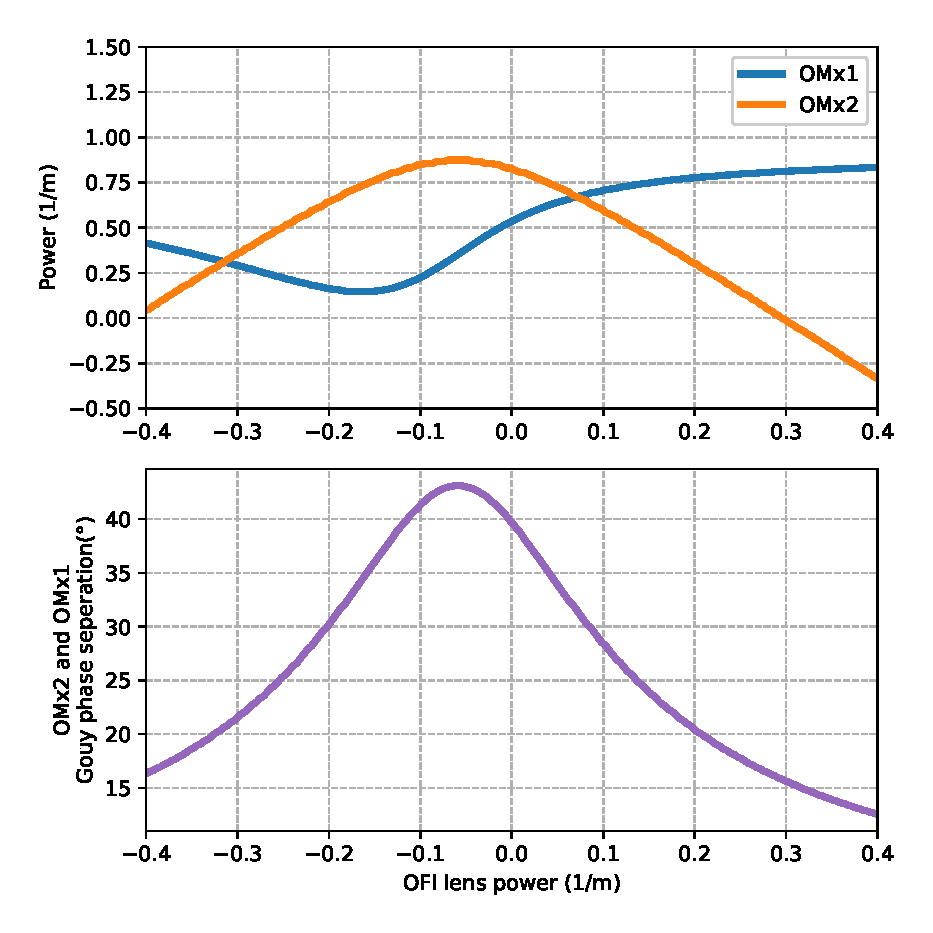
\includegraphics[width=1\linewidth]{Figures/BHD_for_ligo_chapter_lens_choice}
	\caption[Combinations of optical powers for the OFI lens, OMx1 and OMx2 that match the interferometer to the output mode cleaners.]{Top panel: the power of the \gls{ofi} lens power affects the combination of OMx1 and OMx2 powers that is required for 100\% mode matching. Bottom panel: the best choice for the \gls{ofi} lens is where the Gouy phase separation between OMx1 and OMx2 is closest to \ang{45}, as this means OMx1 and OMx2 are as close to being orthogonal as possible. The most Gouy phase separation between OMx1 and OMx2 achievable with this layout is \ang{42}.}
	\label{fig:bhdforligochapterlenschoice}
\end{figure}
\par
As astigmatism degrades the mode matching, it can contribute to the loss in the readout of the interferometer. Astigmatism arises when a beam reflects from a surface with a non-zero angle of incidence; the amount of astigmatism introduced to the beam depends on the beam's curvature and the curvature of the reflecting surface. As the beam in this layout has a relatively low radius of curvature at each mirror, the dominant source of astigmatism is the mirrors (for a comprehensive description of astigmatism see ~\cite{Kochkina:2013bba}). For this layout, the astigmatic loss was calculated to be less than $0.05\%$; see Appendix~\ref{app:mode_matching_algorithm_derivation} for detail in this type of calculation. The astigmatic loss is plotted as a function of angle in Figure~\ref{fig:bhdforligochapterastigmatism}; as the beam will have low curvature, the loss only becomes significant when the angle of incidence is above \ang{10}. Table~\ref{tab:HAM6_losses} summarises the loss budget for the HAM6 layout, and a loss of less than $0.05\%$ is negligible compared to the loss expected from other components.
\begin{figure}
	\centering
	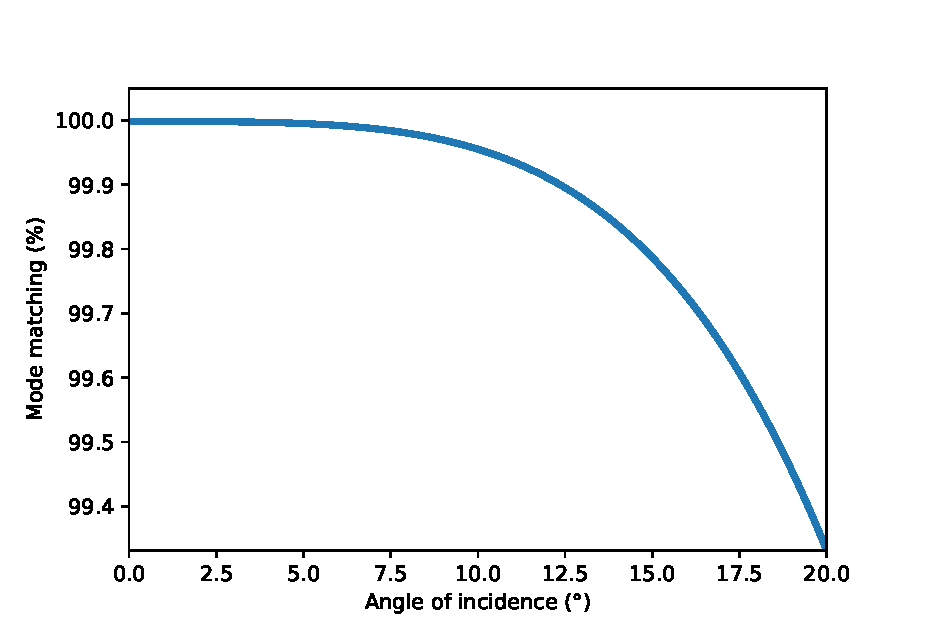
\includegraphics[width=1\linewidth]{Figures/BHD_for_ligo_chapter_astigmatism}
	\caption[Loss due to astigmatism as a function of angle of incidence upon the mirrors for mode matching in HAM6.]{Astigmatism is a source of loss. When designing the layout shown in Figure~\ref{fig:bhdforligochapterlayout5f}, the angle of incidence for the curved mirrors was altered to explore how sensitive it was to astigmatism. Using Equation (\ref{eq:bhd_for_ligo_mm_loss}), the loss was computed. This effect is negligible up to 10\si{\degree}. Above 10\si{\degree}, loss due to astigmatism starts to become significant compared to the losses summarised in Table~\ref{tab:HAM6_losses}.}
	\label{fig:bhdforligochapterastigmatism}
\end{figure}
\par
The Gaussian width and Gouy phase of the beam as a function of position along the optical axis is shown in Figure~\ref{fig:bhdforligochapterbeamshape}. Significant points along the optical axis are also shown in this figure. The size of the beam at the final optic for mode matching matches the size of the target mode, as the size of the beam cannot be changed at a mirror's surface.% The beam is always less than 1.2\,mm within HAM6, an important fact to remember when considering how close structures can be to the beam path; to minimise scattering, the clear aperture size for the beam is defined to be ten times larger than the Gaussian beam width.
\begin{figure}
	\centering
	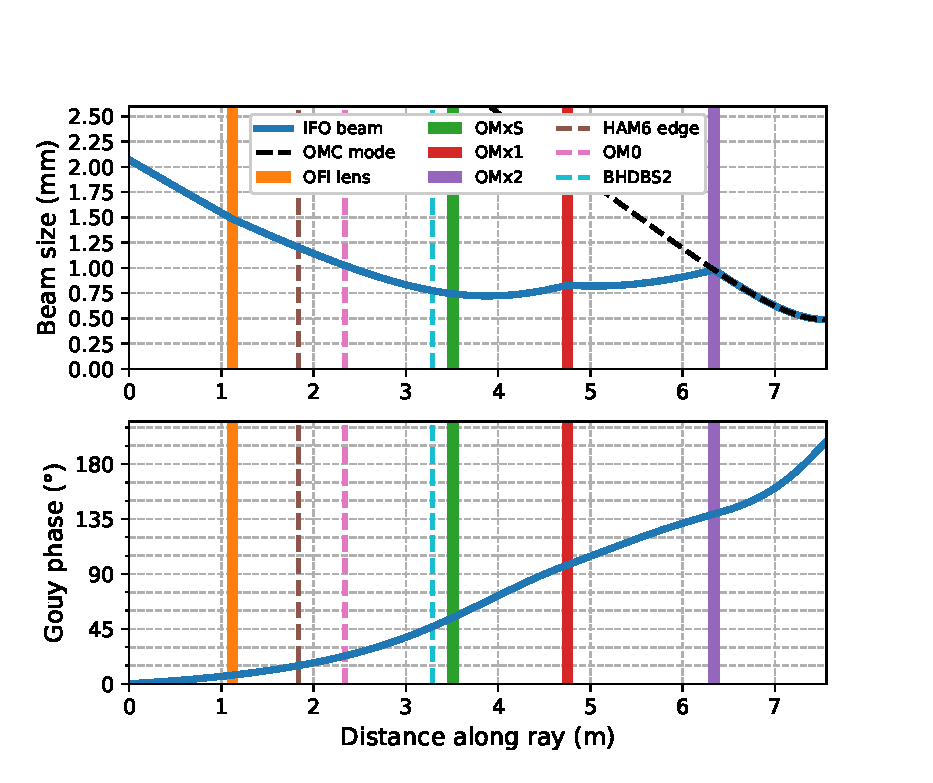
\includegraphics[width=1\linewidth]{Figures/BHD_for_ligo_chapter_Beamshape}
	\caption[Beam size and Gouy phase within HAM6.]{The top panel shows the radius of the beam as it travels from the \gls{srm} (z = 0) to the waist of the \gls{omc}. Significant points along the axis are marked with vertical lines. Less significant, but useful, reference points are marked by dashed vertical lines. The bottom panel shows the Gouy phase shift accumulated by the beam as it propagates along the optical axis.}
	\label{fig:bhdforligochapterbeamshape}
\end{figure}
%\par
%The \gls{omc} design developed for aLIGO~\cite{OMC_ligo}, with trivial modifications, will be used to remove junk light from the signal beam and so there is no choice in target waist size. The nominal \gls{omc} waist size is \SI{485}{\micro\metre}. The beam enters the \gls{omc} through a flat mirror, and a waist is located 140\,mm from this mirror. There is a negligible amount of astigmatism inherent in the design of the \gls{omc}. Optics for mode matching therefore have to match the nominal \gls{srm} and \gls{omc} modes.
\par
%In conclusion, the proposed HAM6 layout is shown in Figure~\ref{fig:bhdforligochapterlayout5f}, and near-orthogonal mode matching control can be achieved with this layout. More comprehensive descriptions of the other aspects of this layout and its requirements can be found in~\cite{CDR_BHD,BHD_ISC_requirements}. A summary of the properties of the layout can be found in Table~\ref{tab:layout_parameters}.
%\clearpage
\begin{table}
	\centering
	\begin{tabular}{| c | c | c | c | }
		\hline 
		Optic & Power (1/m) & Focal length (m) & \gls{roc} (m) \\
		\hline 
		\gls{ofi} lens & -0.066 & -15.068 & -\\
		OMx1 & -0.350 & -2.855 & 5.709 (concave)\\
		OMx2 & -0.847 & -1.180 & 2.360 (concave)\\
		\hline
		\multicolumn{4}{c}{}\\
		\hline
		\multicolumn{2}{|c|}{Space Name} & \multicolumn{2}{|c|}{Optical Path Length (mm)}\\
		\hline
		\multicolumn{2}{|l|}{\gls{srm} to \gls{ofi} lens} & \multicolumn{2}{|c|}{1120}\\
		\multicolumn{2}{|l|}{\gls{ofi} lens to HAM6 table edge} & \multicolumn{2}{|c|}{720}\\
		\multicolumn{2}{|l|}{HAM6 table edge to OM0} & \multicolumn{2}{|c|}{500}\\
		\multicolumn{2}{|l|}{OM0 to BHDBS2} & \multicolumn{2}{|c|}{946}\\
		\multicolumn{2}{|l|}{BHDBS2 to OMxS} & \multicolumn{2}{|c|}{Path A: 225, Path B: 315}\\
		\multicolumn{2}{|l|}{OMxS to OMx1} & \multicolumn{2}{|c|}{Path A: 1240, Path B: 1150}\\
		\multicolumn{2}{|l|}{OMx1 to OMx2} & \multicolumn{2}{|c|}{1590}\\
		\multicolumn{2}{|l|}{OMx2 to OMCx waist} & \multicolumn{2}{|c|}{1220}\\
		\hline
		\multicolumn{4}{c}{}\\
		\hline
		\multicolumn{2}{|c|}{Parameter} & \multicolumn{2}{|c|}{Value}\\
		\hline
		\multicolumn{2}{|c|}{\gls{srm} Complex Beam Parameter} & \multicolumn{2}{|c|}{$q_{\rm{SRM}} = (-3.55 + 1.09i)\,\rm{m} $}\\
		\multicolumn{2}{|c|}{\gls{omc} waist} & \multicolumn{2}{|c|}{485\,\si{\micro\meter}}\\
		\multicolumn{2}{|c|}{OMx1 to OMx2 Gouy phase} & \multicolumn{2}{|c|}{\ang{42}}\\
		\multicolumn{2}{|c|}{OMxS to OMx2 Gouy phase} & \multicolumn{2}{|c|}{Path A: \ang{85}, Path B: \ang{81}}\\
		\multicolumn{2}{|c|}{OMx1 and OMx2 angle of incidence} & \multicolumn{2}{|c|}{A: \ang{9.7}, B: \ang{4.9}}\\
		\hline
	\end{tabular}
	\caption[Mechanical and optical properties of the LIGO A+ HAM6 layout.]{Mechanical and optical properties of the LIGO A+ HAM6 layout.}
	\label{tab:layout_parameters}
\end{table}
\clearpage
%\section{The Requirements for the Optical Layout Within HAM6}
%\label{sec:BHD_for_ligo_layout_requirements}
%The BHD optical layout in HAM6 is required to provide a readout of the gravitational wave signal. To meet the design sensitivity of A+, HAM6 must house a layout that is robust to mode mismatch as there is significant uncertainty in the beam parameter of the arm cavity mode at the SRM. Having control over the two degrees of freedom associated with mode matching -- the size and location of the beam's waist -- between the \gls{omc} and the beam exiting the SRM was challenging as this requires a lot of space relative to the size of the optical table. In addition to this, the HAM6 layout needs to leave space for the other sensors and beams used for controlling the interferometer. All considered designs used most of the available space in HAM6. This section focusses on the design considerations relating to mode matching; other aspects of the functionality required from HAM6 is summarised in~\cite{BHD_ISC_requirements}.
%\par
%To reach the desired level of squeezing, a 2\% mode mismatch is budgeted for to reach the design sensitivity of the A+ detectors. The losses due to components in HAM6 are summarised in Table~\ref{tab:HAM6_losses}~\cite{A+HAM6_design_requirements}. After BHDBS2, the layout should have a pair of mirrors separated by 90\si{\degree} of Gouy phase and another pair separated by 45\si{\degree} of Gouy phase to provide orthogonal control over the beam pointing and mode matching. %The 45\si{\degree} Gouy phase separation requirement makes the design of HAM6 a considerable task. 
%\par
%To reach the desired level of squeezing for A+, the goal for mode matching between the arm mode and the \gls{omc} mode is $>98\%$; the loss contribution of the components in the readout train of the interferometer are summarised in Table~\ref{tab:HAM6_losses}~\cite{A+HAM6_design_requirements}. The loss in sensitivity from mode mismatch can be four times greater than a simpler source of loss (e.g.~photodiode quantum efficiency) due to coherent destructive modal interference~\cite{McCuller2020a} (see Section~\ref{sec:beam_parameter_chapter_mm_losses}). Active mirrors, called Suspended Active Matching Stages (\gls{sams}), will be used to correct for mode mismatch; they will provide at least $\pm50$\,mD of optical power tuning range~\cite{SAMS_DesignRequirementsDocument}.
%\par
%The \gls{awc} in HAM6 has two functions: it will be used to correct for thermal effects in other parts of the interferometer~\cite{BHD_ISC_requirements} such that the mode matching between the arm mode and the \gls{omc} is maximised, and it will be used to correct for \gls{roc} errors in the interferometer after the main beamsplitter. 
%\par
%Thermal changes in the arm cavity mode may be corrected for by the thermal compensation system (TCS)~\cite{Lawrence2002}. However, in practice operators and commissioners use each tunable aspect of the interferometer to improve its sensitivity to gravitational waves. For instance, at \gls{llo} it has been found that TCS can be used to decrease laser intensity noise coupling to DARM~\cite{Blair_email_2020}. As each interferometer subsystem may not be used for its intended purpose, having redundancy in the design of the interferometer is desirable if unexpected noise couplings are discovered. As TCS is used to decrease a noise coupling, it may not be able to correct thermally-driven errors in the arm mode. The optical layout and \gls{awc} functionality in HAM6 were designed with this flexibility in mind. 
%\subsubsection{Gouy phase Separation Between the Optics for mode matching}
%\par
%Two curved mirrors (OMx1 and OMx2) are required to control the two degrees of freedom associated with mode matching. To gain flexibility in the design, a lens will be used to provide further Gouy phase separation between the two active mode matching mirrors in each path after BHDBS2. There is space for this lens on the \gls{ofi} assembly; this is vibrationally isolated and is a useful distance from the optics for mode matching in HAM6. An active lens was considered here, but concerns of \gls{ofi} assembly heating~\cite{A+_Output_Faraday_Isolator_Final_Design} and the unavailability of suitable flint glass meant that this idea was discarded.
%\par
%To provide orthogonal mode matching control, the two \gls{sams} need to be separated by \ang{45} of Gouy phase. Due to the design of the \gls{omc}, the Rayleigh range of the beams in HAM6 are of the order of one meter. As most of the Gouy phase is accumulated within one Rayleigh range either side of a beam waist, a beam will have to travel a significant distance across the table before it acquires sufficient Gouy phase. This Gouy phase separation requirement gave us a method of generating candidate designs as this requirement can be interpreted as needing the mode matching mirrors to be as far apart as possible from each other on the HAM table. Losses due to astigmatism prevents one from using a large angle of incidence to increase the separation between optics in HAM6.
%\par
%Orthogonal alignment control is obtained by having two mirrors separated by \ang{90} of Gouy phase. For all designs, the two mirrors for alignment were immediately after BHDBS2 and immediately before the \gls{omc} as this gave the best Gouy phase separation between them. It was found that placing the first mirror close to BHDBS2 often provided good layouts. References~\cite{CDR_BHD,Webster2020} describes how the longitudinal and pointing degrees of freedom associated with BHD may be sensed and controlled.
%\subsubsection{Readout Platform Suspension and Auxillary Components}
%\par
%The \glspl{omc} are expected to be the largest contributor of back-scatter from HAM6 to the interferometer~\cite{BHD_ISC_requirements,OMC_ligo}; as described in\cite{OMC_ligo}, backscatter can degrade the sensitivity of the interferometer. A single stage suspended platform (BHSS) is required to prevent backscatter noise from reducing the interferometer's sensitivity. Both \glspl{omc} will need to be on this platform and so all designs need to have the \glspl{omc} fairly close to each other. A large BHSS is mechanically infeasible as it will reduce space for the other components on the HAM6 table.
%\par
%Sensors in HAM6 are required to control the alignment between the local oscillator and signal beam, the differential hard mode~\cite{Barsotti2010}, and the alignment between the squeezer and signal beam. These are shown in Figure~\ref{fig:bhdforligochapterlayout5f}. The alignment between the signal and local oscillator beams will be monitored using beams which are picked off from the main beam path and so additional mirrors will be required to steer these beams around the chamber. A set of smaller optics will be installed to provide diagnostic beams which can be imaged with CCD cameras. A shutter will be required to protect the hardware in HAM6 from being damaged by the large amounts of light that can potentially be transmitted through the SRM. 
%\subsection{Fixed Properties of the HAM6 Optical Layout}
%There are a few properties of the HAM6 layout that will not be changed. These include: the entry point of beams into the HAM6 chamber, the size of the nominal mode entering HAM6 and the size of the \gls{omc} waist. Table extensions can be made in places where they would not impede access, however the size of the HAM optical table does restrict the design. It was decided that the two beam paths after  BHDBS2, the optic on which the LO and signal is combined, would be as similar as possible as both beams need to be matched to \glspl{omc} of the same design.
%\par
%As discussed in Chapter~\ref{chapter:simulation_finesse}, the beam parameter at the SRM is expected to differ from its nominal value of $q_{\rm{SRM}} = -3.55 + 1.09i\,\rm{m} $~\cite{AS_port_beam_parameter}. It is described in Chapter~\ref{chapter:simulation_finesse} how geometry errors in the \gls{src} cause the arm cavity and the \gls{src} to be mismatched. From this, a set of modes which may be present at the SRM was calculated. The design of the layout within HAM6 is based on the nominal beam parameter, and the set of modes shown in Figure~\ref{fig:sim_chapter_beam_parameter_at_SRM} was taken into consideration when analysing the pros and cons of different candidate layouts since they may have been more or less robust to beam parameter errors at the SRM. 
%\par
%The \gls{omc} design developed for aLIGO~\cite{OMC_ligo}, with trivial modifications, will be used to remove junk light from the signal beam and so there is no choice in target waist size. The nominal \gls{omc} waist size is \SI{485}{\micro\metre}. The beam enters the \gls{omc} through a flat mirror, and a waist is located 140\,mm from this mirror. There is a negligible amount of astigmatism inherent in the design of the \gls{omc}. Optics for mode matching therefore have to match the nominal SRM and \gls{omc} modes.
%\par
%\subsubsection{Equal Path Lengths after BHDBS2}
%It was decided that the two beams after BHDBS2 would have the same path length to reduce the cost of the HAM6 optics. This may also improve the common-mode noise rejection ratio as asymmetries may enhance the effects of noise couplings. To achieve high levels of common mode noise rejection, both paths should be as similar as possible. Only one path needs to have imperfections for the common mode rejection ratio to be degraded. For instance, it may be a bad design choice to have a path with a mirror whose only purpose is to fold the layout so that a slightly better readout platform can be used. However, it should be noted that the amount of common mode rejection required is related to the classical noise of the laser and its shot noise limit. Since the LO in LIGO A+ will be derived from the PRC it will already be stable \textcolor{red}{(shot noise?)}, so little common mode noise rejection will be needed. \textcolor{red}{ In addition to this, the layout will be in a clean environment with a low amount of residual gas; thus reducing mechanisms whereby imbalances due to path length difference can generate noise (may remove?)}. Therefore, the trade-off between mirror number and path length symmetry versus readout platform preference is not necessarily easy to evaluate.   
%\subsection{Summary}
%HAM6 must contain a layout which combines the local oscillator and the signal beam. The loss due to mode matching must be $<2\%$  The optical layout within HAM6 constitutes a nontrivial design task as it is desirable to have orthogonal control over the mode matching and beam direction. This requires the optical axis to be of a similar length as the maximum spacing permitted by a HAM table. In addition to this, the HAM6 layout needs to leave space for all the other sensors and beams used for control. This means that all designs will use nearly all of the table space.
\begin{table}[ht]
	\centering
	\begin{tabular}{| l | c |}
		\hline
		HAM6 loss Source & Target for O5 \\
		\hline
		\gls{omc} throughput loss & $<2\%$ \\
		OM3 transmission (or equivalent) for sensing & 1--2\% \\
		Photodiode quantum efficiency & 1\% \\
		Mode mismatch to the \gls{omc} & $<2\%$ (as low as possible) \\
		Any other optical loss & $<1\%$\\
		\hline
	\end{tabular}
	\caption[Target for losses in HAM6.]{Target for losses in HAM6. Reproduced from~\cite{A+HAM6_design_requirements}.}
	\label{tab:HAM6_losses}
\end{table}
\section{Method for Visualising the Effectiveness of Systems with Active Optics for Mode Mismatching}
\label{sec:BHD_for_ligo_WS_visulations}
As described in Section~\ref{sec:bhd_for_ligo_chosen_layout} and Chapter~\ref{chapter:simulation_finesse}, it is expected that there will be some mismatch between the arm mode and the \gls{omc}. To visualise the effectiveness of the \gls{awc} provided by the layout's active optics, it is useful to consider a 2D space representing Gaussian beams. The region of this space which contains modes that can be matched to >98\% by the \gls{awc} and a distribution of modes that those optics may have to correct for can be compared to gain insight into the effectiveness of the layout. 
\par
The proposed layout in Section~\ref{sec:bhd_for_ligo_chosen_layout} can mode match the majority of beam parameters one would expect to be present at the \gls{srm} based on uncertainties in the \gls{roc} of the optics within the \gls{src}. Despite this good coverage, measurements from \gls{llo} show that the beam parameter may fall outside the region of \gls{ws} space which can be compensated for by the layout. If this were the case, the static \gls{roc} of the \gls{sams} would need to be changed.
\subsection{A Description of Mode Matching in Terms of Hermite-Gaussian Modes}
%The mode matching between two laser beam modes, or a laser mode and a cavity mode, describes how similar those two modes are. In general, a combination of misalignment and differing beam shape can be considered to be a mode mismatch. However, mode matching typically refers to the overlap of the two modes if they were co-aligned, thus it is a measure of how similar in shape the two modes are. Mode matching between two modes is usually, to first approximation, thought of as a difference in their waist size and waist location.
%\par
Beams which are mode matched have identical beam parameters, i.e.~they have the same sized waist and their waists are at the same position along the optical axis. Small mode mismatches can be modelled as light scattering from the beam's, or cavity's, fundamental mode into its $\rm{HG}_{20}$ and $\rm{HG}_{02}$ modes (i.e~the $\rm{HG}_{20+02}$ mode). If a cavity is designed such that the fundamental mode will be resonant while the $\rm{HG}_{20+02}$ mode will be reflected, the effect of mode mismatch between the cavity and a signal carrying beam is to decrease the signal light that is transmitted by the cavity since some of the signal carrying light will be scattered into the reflected $\rm{HG}_{20+02}$ mode. Sensing the $\rm{HG}_{20+02}$ mode therefore gives a measure of the mode matching between two modes. As the $\rm{HG}_{20+02}$ mode acquire $2\phi$ Gouy phase compared to the fundamental mode, where $\phi$ is the Gouy phase acquired by the fundamental mode, spacing beam curvature actuators at \ang{45} of Gouy phase apart provides an orthogonal basis for control over mode matching~\cite{Morrison1994}.

%\par
%A change in waist size is equivalent to an in-phase coupling between the fundamental mode and the $\rm{HG}_{20} + \rm{HG}_{02}$ modes, whereas a change in waist location is a coupling to the $\rm{HG}_{20} + \rm{HG}_{02}$ modes which is \ang{90} out of phase with the fundamental mode~\cite{Morrison1994}. As the $\rm{HG}_{20} + \rm{HG}_{02}$ modes acquire $2\phi$ compared to the fundamental mode, where $\phi$ is the Gouy phase acquired by the fundamental mode, spacing beam curvature actuators at \ang{45} will give an orthogonal basis for control over mode matching. Orthogonal control results in the beam size and beam waist, or two combinations of them that are orthogonal, can be independently controlled.
\subsection{Calculating Mode Matching Using The Gaussian Beam Parameter}
Two perfectly mode matched beams will have identical beam parameters at the same point along the optical axis. The overlap integral between two fields, $E_1$ and $E_2$,
\begin{equation}
\mathcal{M} = \frac{\left|\int_{A} E_1^*E_2 dA \right|}{\int_{A} \left|E_1 \right|^2 dA \int_{A} \left|E_2 \right|^2 dA},
\label{eq:bhd_for_ligo_mode_matching_general}
\end{equation}
can be used to determine the amount of mode matching, $\mathcal{M}$, between two astigmatic modes. Solving this integral gives
\begin{equation}
\mathcal{M} =\frac{\sqrt{\big(q_{x1}-q_{x1}^*\big)\big(q_{y1}-q_{y1}^*\big)\big(q_{x2}-q_{x2}^*\big)\big(q_{y2}-q_{y2}^*\big)}}{\big|q_{x2} - q_{x1}^*\big|\big|q_{y2} - q_{y1}^*\big|},
\label{eq:bhd_for_ligo_mm_loss}
\end{equation}
where $q_{x1,x2,y1,y2}$ are the beam parameters of the electric fields $E_{1,2}$ in the tangential and sagittal planes. This is derived in Appendix~\ref{app:mode_matching_algorithm_derivation}. The solution to Equation (\ref{eq:bhd_for_ligo_mm_loss}) is always $0<\mathcal{M} \leq 1$. Alternatively, mode matching may be computed in terms of the amplitude of the higher order modes relative to the fundamental mode~\cite{Bayer-Helms1984}. The mode matching can be calculated at any point along the optical axis of the layout because mode matching must be preserved throughout it; however, it makes sense to calculate the mode matching in a physically significant plane such as the input plane, a plane containing a curved optic or the plane containing the waist of the target beam.
\subsection{Waist-Defocus Phase Space Visualisations}
A Gaussian beam can be described by its beam size, $w$, and defocus, $S$~\cite{Perreca2020}. A \gls{ws} phase space representation plots a Gaussian beam in terms of these two parameters. The effect of focussing elements on Gaussian beams can be clearly seen in this representation of them. Because a curved mirror can only change the curvature of a beam, at the mirror's surface the beams before and after reflection must have the same size. The process of a Gaussian beam, described by $q_1(S_1,w_1)$, being reflected from a mirror with power $S_{\rm{m}}$ to produce a new Gaussian beam, $q_2$, can be written as
\begin{equation}
\frac{1}{q_2} = S_{\rm{m}} + \frac{1}{q_1} = (S_{\rm{m}}+S_1) - i\frac{\lambda}{\pi w_1^2}.
\label{eq:BHD_for_ligo_2_1_over_q}
\end{equation}
From Equation (\ref{eq:BHD_for_ligo_2_1_over_q}) it can be seen that a mode moves in the $S$ direction when it reflects from a curved mirror. This representation of Gaussian beams has the advantage of showing the beam in terms of intuitive quantities. The downside to this representation is as the beam propagates through the layout, the path that is traced through the \gls{ws} space by the mode is fairly complicated. 
\par
There are two other ways that a beam parameter could be graphically represented. Since $q$ is a complex number, it could be represented in terms of its real and imaginary components. This makes seeing the effect of propagation straight forward, but the effect of a focussing element is harder to visualise. Alternatively, plotting $1/q$ in terms of $\lambda/\pi w^2$ and $S$ produces plots where the effect of focussing elements and propagation are easy to visualise~\cite[p.680]{lasers1986}. Curved mirrors and lenses result in a change in defocus, and propagated modes follow circular paths. As these figures are being used to visualise mode matching and the effect of actuators on the beam size (rather than $\lambda/\pi w^2$) and defocus, the \gls{ws} representation was chosen. One could express the beam parameter in terms of natural units by dividing the beam size by the beam's minimum waist size, $w_0$, and the defocus by the inverse of the beam's Rayleigh range, $1/z_R$.
\par
To illustrate how actuators move a mode in \gls{ws} space, consider two lenses with variable power separated by \ang{45} of Gouy phase, thus making them orthogonal. In a \gls{ws} space, the orthogonality of two actuators can be seen by the angle between the two vectors that represent each actuation. Figure~\ref{fig:bhdforligochapterwssketch} is a sketch of the \gls{ws} space representation for a simple optical layout consisting of two active lenses separated by \ang{45} of Gouy phase.
\begin{figure}
	\centering
	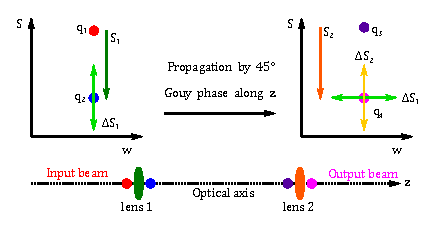
\includegraphics[width=0.95\linewidth]{Figures/BHD_for_ligo_chapter_WS_sketch}
	\caption[Sketch of the waist-defocus representation for a Gaussian beam interacting with a simple optical layout.]{Sketches of the \gls{ws} representation for a Gaussian beam interacting with different parts of a simple optical layout consisting of two active lenses with powers $S_{1,2} \pm \Delta S_{1,2}$. The left-hand axes shows the \gls{ws} plane at Lens 1. The input beam, $q_1$, is indicated by a red dot, and the effect of the lens on $q_1$ is shown by the dark green arrow $S_1$. This results in a new mode $q_2$ which is shown as a blue dot. A light green arrow indicates the actuation of Lens 1. The right-hand axes shows the \gls{ws} plane at Lens 2. The input mode at Lens 2, $q_3$, is shown as a purple dot, and the output mode, $q_4$, is shown as a pink dot. The static and dynamic power of Lens 2 is indicated by the orange and yellow lines. As Lens 1 and Lens 2 are separated by $45\si{\degree}$ of Gouy phase, the actuation provided by Lens 1 results in a change in the beam parameter which is orthogonal to the actuation provided by Lens 2, provided that the actuations are small enough. Beneath the two \gls{ws} space diagrams is a sketch of the optical axis and the location of the modes.}
	\label{fig:bhdforligochapterwssketch}
\end{figure}
\par
It is useful to plot contours of the mode overlap in the \gls{ws} space between a mode and a target mode. Note that these contours can only tell you about the overlap between a mode and the target mode; the mode matching between two arbitrary modes can not be deduced from these contours~\cite{Perreca2020}. For example, two modes may be mismatched by the same amount from the target in orthogonal directions in \gls{ws} space. They cannot be perfectly mode matched as these two modes are different from each other.
\subsection{Visualising how the Active Optics for Mode Matching Expand the Area of Waist-Defocus Space Representing Acceptable Input Modes}
To visualise the effectiveness of the actuation provided by the active elements of the HAM6 layout, the region of the \gls{ws} space at the \gls{srm} from which the target mode matching space can be achieved was computed. To do this, first the ring of modes in \gls{ws} space that is $98\%$ mode matched to the \gls{omc} after reflection from the second active mirror, OMx2, was considered. If OMx2 had a static radius of curvature, the effect of OMx2 would be to move the ring vertically in the \gls{ws} plane. However, the ring can also be stretched in the $S$ direction as OMx2's \gls{roc} can be changed. This can be seen, crudely, by applying $S_{\rm{OMx2}}\pm\Delta S$ to the original $>98\%$ mode matching ring to produce two new rings separated by $2\Delta S $. 
\par
To generate the region from which the target region can be reached by OMx2, the target region should be cut by a line which intersects the ring at the extrema of the beam size. To maximise the amount of \gls{ws} space covered by the actuator, the upper target region should have $+\Delta S$ applied to it whereas for the lower region the actuation should be $-\Delta S$. This results in a region of \gls{ws} space which is larger than the initial target region. All modes in the new region can be at least $98\%$ mode matched to the \gls{omc}. The new region was then propagated to the first mirror, OMx1, where the same procedure can be applied to further expand the region. This process is shown in Figure~\ref{fig:bhdforligochapterlayout5fomx1omx2planes}.
\begin{figure}
	\centering
	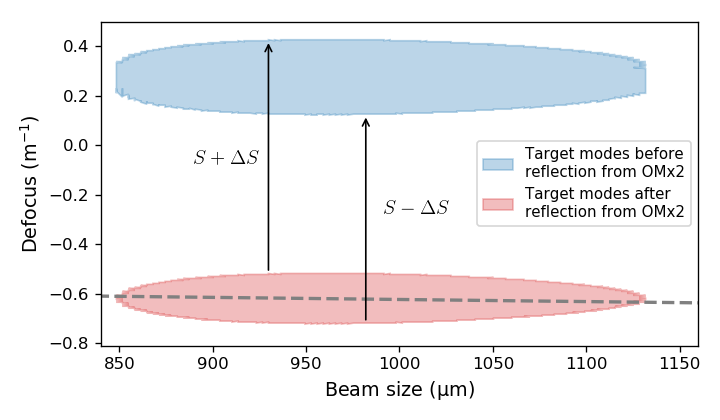
\includegraphics[width=1\linewidth]{Figures/BHD_for_ligo_chapter_layout_5f_omx1_omx2_planes.png}
	\caption[Sketch showing how the expansion of the area of waist-defocus space by active optics is computed.]{The \gls{ws} space at the OMx2 plane. The effect of OMx2 in the plane of OMx2 is to move a mode vertically in \gls{ws} space. After reflection from OMx2, a mode should be at least $98\%$ mode matched to the \gls{omc} as there are no further active mode matching elements in the layout of HAM6. Such modes are shown by the red region. The blue region represents modes which can be reached from the red region by either $S_{\rm{OMx2}}\pm\Delta S$, and was constructed by applying transformations to the modes in the red region. The red region was split into two parts, `upper' and `lower', indicated by the dashed line that connects the two extremes in width of the region. To create the lower edge of the blue region, modes in the lower edge of the red region had the transformation corresponding to a mirror power of $S_{\rm{OMx2}}-\Delta S$ applied to them. To construct the upper edge of the blue region, the upper edge of the red region had the transformation corresponding to a mirror power of $S_{\rm{OMx2}}+\Delta S$ applied to them.}
	\label{fig:bhdforligochapterlayout5fomx1omx2planes}
\end{figure}
\begin{figure}
	\centering
	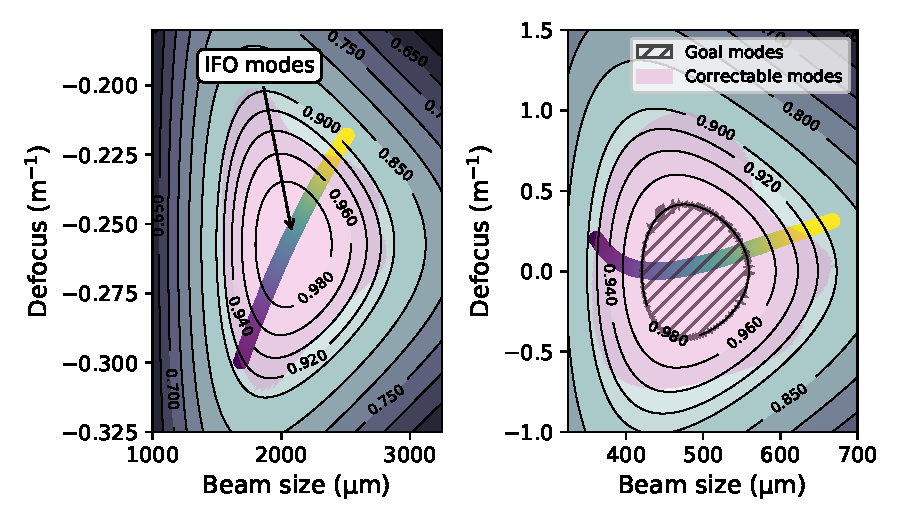
\includegraphics[width=1\linewidth]{Figures/BHD_for_ligo_chapter_layout_5f_Modes_srm_omc_mode_matching_success.pdf}
	\caption[Coverage of the waist-defocus space provided by the active optics for mode matching in HAM6.]{The region of \gls{ws} space covered by the \gls{awc} in HAM6 for the layout discussed in Section~\ref{sec:bhd_for_ligo_chosen_layout}. Left panel: the set of modes that is expected to be present at the \gls{srm}, as described in Chapter~\ref{chapter:simulation_finesse}, is shown by the purple-blue-green-yellow curve. The pink region shows which modes can be corrected for so that 98\% mode matching is achieved. The contours indicate the mode matching between a mode $(W,S)$ and the \gls{omc} mode. The red cross indicates the mode size that can be inferred from measurements of the \gls{src}'s Gouy phase at \gls{llo}. Right panel: this shows the same modes as the left panel, except they have been transformed by the optical layout to the plane of the \gls{omc} waist. Modes within the pink region can be actuated on so they move to the goal region, which is indicated with a hatched area.}
	\label{fig:bhdforligochapterlayout5fmodessrmomcmode matchingsuccess}
\end{figure}
\par
The modes from the \gls{srm} that can be matched to the target are shown in Figure~\ref{fig:bhdforligochapterlayout5fmodessrmomcmode matchingsuccess}. To visualise how successful the layout is at handling the likely modes from the interferometer (i.e.~the set of modes investigated in Chapter~\ref{chapter:simulation_finesse}), the interferometer modes were compared to the region of \gls{ws} space containing modes which can be corrected such that they meet the $>98\%$ mode matching requirement. It was found that majority of likely modes will be covered by the layout as the modes near the edge of the interferometer mode continuum are more unlikely to occur than the ones near the centre; however, measurements of the \gls{src}'s Gouy phase at \gls{llo} can be used to infer the beam parameter at the \gls{srm}, and this mode would fall outside of the region of \gls{ws} space which can be compensated for by the \gls{awc}. Its worth noting that the modes at the yellow end of the continuum shown in Figure~\ref{fig:bhdforligochapterlayout5fmodessrmomcmode matchingsuccess} may not be physical as they correspond to an unstable \gls{src}.
%\par
%For all candidate layouts analysed there was no major difference in the amount of modes that could be mode matched.  In principle, the requirement for having \ang{45} of Gouy phase separation between OMx1 and OMx2 does not maximise the amount of \emph{likely} interferometer modes that can be mode matched. It is be possible to shape the region of \gls{ws} space covered by the layout to maximise the probability that the arm mode will be at least 98\% mode matched to the \gls{omc} by the layout. For example, if it was found that arm modes were most likely to be characterised by an error in beam waist size at the \gls{omc}, the active optics should be arranged so that they can actuate predominantly on beam size at the \gls{omc}. However, choosing a layout which favours flexibility in one degree of freedom over the other may lead to unforeseen beam parameter errors being uncorrectable.
\par
The shape of the pink region in Figure~\ref{fig:bhdforligochapterlayout5fmodessrmomcmode matchingsuccess} is nominal; when the HAM6 layout is constructed the pink region's shape will be altered by geometric errors in OMx1 and OMx2. Nevertheless, Figure~\ref{fig:bhdforligochapterlayout5fmodessrmomcmode matchingsuccess} is encouraging since it shows that the actuation provided by OMx1 and OMx2 is highly tolerant to mode matching errors generated by errors in the \gls{src}.
\subsection{Optimising Waist-Defocus Space Coverage in Favour of Expected Mode Errors}
\label{sec:BHDforligochapter_super_actuator}
The majority of the uncertainty in the interferometer's beam parameter comes from the uncertainty in SR3's \gls{roc} (see Figures~\ref{fig:beamsizesimulated} and~\ref{fig:beamrocsimulated}). Ideally, one would correct for this by actuating on the \gls{roc} of SR3. While there is no hardware that can actuate on the \gls{roc} of SR3 strongly enough, one could configure the \gls{awc} within HAM6 such that it is biased for correcting the errors in the interferometer's beam parameter caused by the error in SR3. 
\par
By reducing the orthogonality of the \gls{awc} actuators, more range can be obtained for one of the beam's properties, e.g.~the size of its waist. A Gouy phase separation $\sim\!\ang{30}$ offers a compromise between orthogonality versus actuation range for errors in one of the beam parameter's dimensions; for a given Gouy phase, a set of static optical powers can be obtained from Figure~\ref{fig:bhdforligochapterlenschoice} for the \gls{ofi} lens, OMx1 and OMx2 that gives perfect mode matching between the interferometer's nominal beam parameter and the \glspl{omc}. However, layouts with less Gouy phase separation between OMx1 and OMx2 also have less Gouy phase separation between the mirrors for aligning the interferometer to the \glspl{omc}, so this idea was ultimately rejected.

%While \ang{45} of Gouy phase separation between the optics for mode matching in HAM6 is a desirable quality for the layout to have, the layout can be optimised to correct for mode mismatches between the \gls{omc} and the continuum of expected beams exiting the interferometer. The majority of the uncertainty in the interferometer's beam parameter comes from the uncertainty in SR3's \gls{roc} (see Figures~\ref{fig:beamsizesimulated} and~\ref{fig:beamrocsimulated}). 


%By reducing the orthogonality of the AWC actuators, more range can be obtained for one of the beam's property e.g. the size of a beam's waist. A Gouy phase separation ($\sim\!\ang{30}$) offers a compromise between orthogonality versus actuation range for errors in one of the beam parameters dimensions
%\par
%Ideally, one would correct for this by actuating on the \gls{roc} of SR3, however the \gls{roc} of SR3 cannot be strongly actuated on. If a mirror was placed \ang{180} of Gouy phase away from SR3, it could be used to compensate for the uncertainty in the \gls{roc} of SR3 i.e.~one could configure the optics for mode matching within HAM6 such that they are biased for correcting the errors in the interferometer beam parameter caused by the error in SR3. 
%\par
%By reducing the orthogonality of the AWC actuators, more range can be obtained for one of the beam's property e.g. the size of a beam's waist. A Gouy phase separation ($\sim\!\ang{30}$) offers a compromise between orthogonality versus actuation range for errors in one of the beam parameters dimensions. Figure~\ref{fig:bhdforligochapterlayout5fsuperactuator} shows how the region of \gls{ws} space covered by the HAM6 AWC can be biased in favour of the expected set of modes that may emerge from the SRM. The physical positions of the optics are the same as before (see Table~\ref{tab:layout_parameters}), however the optical powers of the \gls{ofi} lens, OMx1 and OMx2 was altered (-0.2, 1.67, 0.631 respectively) to change the Gouy phase separation between OMx1 and OMx2 to \ang{30}. However, the Gouy phase for alignment control would be significantly reduced; this is shown in Figure~\ref{fig:bhdforligochapterbeamshapesa}.
%\begin{figure}
%	\centering
%	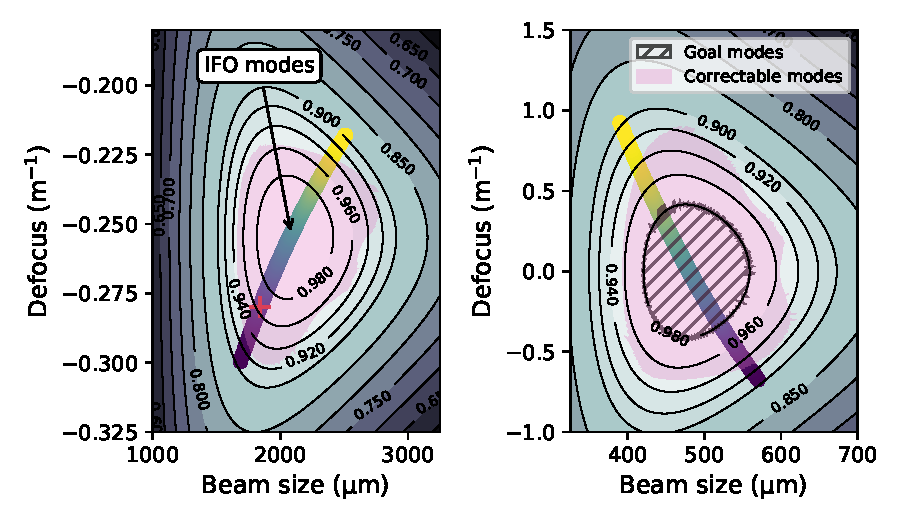
\includegraphics[width=1\linewidth]{Figures/BHD_for_ligo_chapter_layout_5f_super_Actuator}
%	\caption{At the expense of orthogonality, the region of \gls{ws} space covered by the AWC in HAM6 can be optimised by changing the Gouy phase separation between OMx1 and OMx2. Left panel: the set of modes that could be emerge from at the SRM, as described in Chapter~\ref{chapter:simulation_finesse}, is shown by the purple-blue-green-yellow curve. The pink region shows which modes can reach 98\% mode matching by using the AWC in HAM6. The contours indicate the mode matching between a mode $(W,S)$ and the \gls{omc} mode. Right panel: this shows the same modes as the left panel; however, they have been transformed by the optical layout to the plane of the \gls{omc} waist. Modes within the pink region can be actuated on so they move to the goal region (hatched area).}
%	\label{fig:bhdforligochapterlayout5fsuperactuator}
%\end{figure}
%\begin{figure}
%	\centering
%	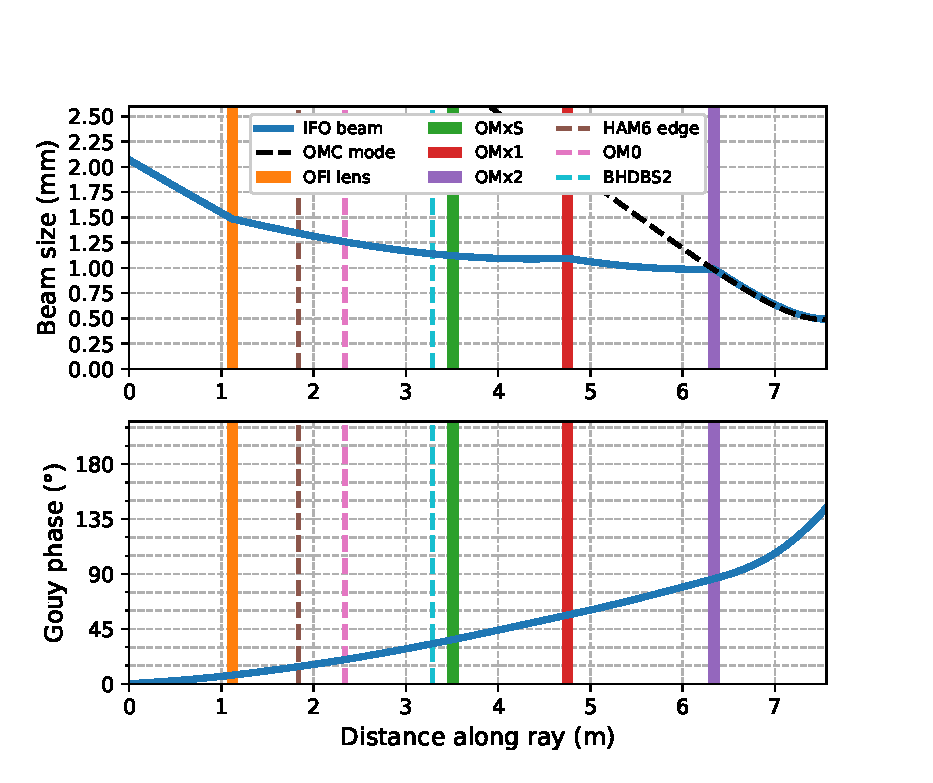
\includegraphics[width=1\linewidth]{Figures/BHD_for_ligo_chapter_Beamshape_SA}
%	\caption{Top panel: the beam profile for the alternative layout of HAM6 suggested in Section~\ref{sec:BHDforligochapter_super_actuator}. Bottom panel: The Gouy phase accumulated along the optical axis for the alternative layout. While alignment Gouy phase is degraded, the mode matching Gouy phase was changed to bias the optical layout for correcting errors in the \gls{roc} of SR3.}
%	\label{fig:bhdforligochapterbeamshapesa}
%\end{figure}
%\clearpage
\section{Conclusion}
\label{sec:BHD_for_ligo_conclusion}
The proposed layout for HAM6 was presented in Section~\ref{sec:bhd_for_ligo_chosen_layout}. The optical properties of this layout were investigated. By selecting the right combination of optics for mode matching, near orthogonal control of the mode matching and alignment between the interferometer and the \gls{omc} can be achieved.
\par
The effect that the \gls{awc} had on the region of \gls{ws} space that contains modes which satisfy the $>98\%$ mode matching requirement was investigated. \gls{ws} diagrams were used to represent how robust the layout is to initial mode mismatch. Figure~\ref{fig:bhdforligochapterlayout5fmodessrmomcmode matchingsuccess} shows the amount of \gls{ws} space that the \gls{awc} could correct for. The \gls{awc} covers a wide range of possible modes that may emerge from the interferometer, and the static defocus of the \gls{sams} can be changed, so it is highly likely that the \gls{awc} in HAM6 will give optimal mode matching between the interferometer and the \gls{omc}. 